\documentclass[11pt,a4paper]{article}
\usepackage[utf8]{inputenc}
\usepackage[T1]{fontenc}
\usepackage[english]{babel}
\usepackage[margin=2.3cm]{geometry}
\usepackage{booktabs,tabularx}
\usepackage{graphicx}
\usepackage{float}
\graphicspath{{docs/references/}{references/}}

\usepackage[hidelinks]{hyperref}
\usepackage{fancyhdr}
\usepackage{listings}
\setlength{\parindent}{0pt}
\setlength{\parskip}{0.45em}
\setlength{\headheight}{14pt}
\pagestyle{fancy}
\fancyhf{}
\fancyhead[L]{Third Progress Report}
\fancyhead[R]{Agent Capability Graph}
\fancyfoot[C]{\thepage}
\lstset{basicstyle=\ttfamily\footnotesize,breaklines=true,columns=fullflexible,keepspaces=true,frame=single}

\begin{document}
\hypersetup{pageanchor=false}
\begin{titlepage}
\centering
\vspace*{1.5cm}
{\LARGE\bfseries MY 4th PROGRESS REPORT\par}
\vspace{1.5cm}
{\Huge Agent Capability Graph\par}
\vspace{0.4cm}
{\Large Building an RDF Knowledge Graph to Discover MCP Servers and Agent Skills\par}
\vspace{1.5cm}
\begin{tabular}{ll}
\textbf{Main Supervisor:} & Raphael Troncy \\
\textbf{Secondary Supervisor:} & Thibault Ehrhart \\
\textbf{Document Type:} & Fourth Progress Report \\
\textbf{Phase:} & Corpus Integration, SPARQL and SHACL Validation \\
\textbf{Reporting Period:} & November 13--20, 2026
\end{tabular}
\vfill
{\large November 20, 2026\par}
\end{titlepage}
\hypersetup{pageanchor=true}

\section{Continuation of last week's work}

In my second progress report, dated November 12, I presented a curated sample of ten MCP servers, forty-three documented tools and ten Agent Skills, together with a SQLite-to-RDF pipeline producing 2,210 triples. The next objectives were to formulate discovery questions, implement SPARQL queries and investigate SHACL validation.

This week, I worked on these objectives and integrated the larger metadata corpus added by my colleague. My main goal was to obtain one coherent graph that could answer concrete questions while preserving the evidence behind each description and capability annotation.

\section{Selecting and integrating the additional metadata}

The expanded snapshot contains 502 MCP server records, seventeen tool records and 272 Skills. I observed that the seventeen tools were documented for only two servers: Filesystem and Brave Search. Including all server records would therefore increase the graph size without providing comparable tool-level information for most of them. This is a limitation of the collected metadata, not evidence that the other servers expose no tools.

I retained the initial sample and selected 100 additional Skills. The selection prioritizes explicit requirements metadata and direct sources associated with repository revisions, excludes identified duplicate content, and alternates between available repositories. The selected additions comprise 95 direct-source records and five secondary imports. I froze the selection in \path{config/corpus_selection.json}, including record fingerprints, so rebuilding does not silently change the sample.

I then reconciled the two sources. Both additional servers already existed in the initial sample, and five tool records matched existing tools. Seven initial Skills also received complementary metadata. I matched tools by canonical server and tool name, and Skills by repository and \texttt{SKILL.md} path, rather than by name alone.

\begin{table}[htbp]
\centering
\caption{Evolution from the previous report to the unified working graph.}
\begin{tabular}{lrr}
\toprule
\textbf{Item} & \textbf{Previous report} & \textbf{Current graph} \\
\midrule
MCP servers & 10 & 10 \\
MCP tools & 43 & 55 \\
Agent Skills & 10 & 110 \\
RDF triples & 2,210 & 6,765 \\
\bottomrule
\end{tabular}
\end{table}

The original observations, source documents and revisions remain available. Selection and identity decisions are exported under \path{reports/corpus/}. This is a deliberately selected research sample, not a representative inventory of all MCP servers or Skills.

\section{Clarifying and implementing capabilities}

A difficulty this week was distinguishing the presence of a resource from the presence of a capability annotation. My first integrated graph contained 110 Skills, but none had an explicit capability assertion. An inventory count of zero therefore indicated missing classification work, not an absence of useful functions.

I clarified a capability as a normalized task, represented by an action and an object, such as \texttt{search / web} or \texttt{process / PDF document}. The resource remains separate from the capability concept. An \texttt{acg:CapabilityAssertion} connects them and records the method, evidence and review status.

I preserved the seventeen assertions based on static tool registrations and added explicit task mappings in \path{config/capability_mappings.json}. For the other tools and Skills, a mapping is applied only when its expected passage occurs in the resource's source description. These are proposed curator mappings, not automatically verified semantic facts. I currently assign a first supported task rather than claiming an exhaustive description of every operation.

For servers, I derive capability assertions from their exposed tools and retain links to the supporting tool assertions through \texttt{acg:derivedFromAssertion}. The graph now contains 149 capability concepts and 210 assertions. All remain candidates for human review.

\section{Implementing the discovery questions in SPARQL}

I implemented query files under \path{queries/} for the questions identified in the previous report.

\begin{itemize}
\item \textbf{Web search tools:} the query follows capability assertions with action \texttt{search} and object \texttt{web}. It retrieves \texttt{brave\_web\_search} with evidence from its pinned registration. Fetching a known URL or searching a specific documentation collection is distinguished from general Web search.
\item \textbf{Skills working with a format:} PDF and spreadsheet searches are separate executions of a parameterized query. They return description-based candidates and aggregate source links per canonical Skill. These matches still require interpretation of exclusions and context.
\item \textbf{Skill requirements:} the query exposes recorded dependencies, compatibility, allowed tools and bundle indicators. For example, \texttt{phoenix-observability} has a recorded dependency on \texttt{arize-phoenix>=12.0.0}, originating from a secondary import. A missing field is treated as unknown rather than proof that no requirement exists.
\end{itemize}

I also added an entity-level query that displays normalized tasks together with their annotation method, review status and evidence.

\section{Adding SHACL validation and preparing human review}

I implemented SHACL validation with pySHACL and separated two checks. Structural shapes verify names, evidence documents, tool-to-server relationships and capability assertions. For derived server claims, a SPARQL constraint verifies that the supporting assertion belongs to an exposed tool and expresses the same task. Coverage shapes separately identify resources without any task assertion.

\begin{table}[htbp]
\centering
\caption{Current annotation coverage; all annotations remain review candidates.}
\begin{tabular}{lrrr}
\toprule
\textbf{Resource type} & \textbf{Total} & \textbf{Annotated} & \textbf{Unclassified} \\
\midrule
MCP servers & 10 & 10 & 0 \\
MCP tools & 55 & 55 & 0 \\
Agent Skills & 110 & 109 & 1 \\
\bottomrule
\end{tabular}
\end{table}

The graph passes structural SHACL validation. Coverage reports one warning for \texttt{template-skill}, whose description is placeholder text. I kept this case visible instead of assigning an unsupported task. Strict validation also fails on incomplete coverage. The implementation is accompanied by 21 automated tests covering selection, evidence preservation, identity merging and negative validation cases.

I generated \path{reports/capabilities/review.csv} to support semantic review. Human review means checking whether the source actually justifies the proposed task and its scope. It is different from structural validation and from executing a tool. No assertion is currently marked as human-reviewed, and persistent review decisions are not yet imported by the pipeline.

\section{Simplifying the project and its workflow}

As the project grew, multiple launchers, historical graphs and duplicate consultation files made the repository difficult to navigate. I consolidated active code under \path{src/acg/}, placed the ontology and shapes under \path{ontology/}, and centralized operations in \texttt{pipeline.py}. JSONL and SQLite remain computation inputs; consultation CSVs are now grouped under \path{reports/}.

I moved obsolete configurations, prototypes, launchers and drafts into \path{archive/}, preserving the project history and recording the moves. I checked that the cleanup preserved the working graph's RDF content. The main offline workflow is now:

\begin{lstlisting}
metadata/.venv/bin/python pipeline.py run
\end{lstlisting}

This builds the selected graph, adds task annotations, prints the inventory and runs SHACL. Collection, normalization and queries remain explicit commands. For example:

\begin{lstlisting}
metadata/.venv/bin/python pipeline.py query tools_for_web_search.rq
\end{lstlisting}



\begin{figure}[H]\centering
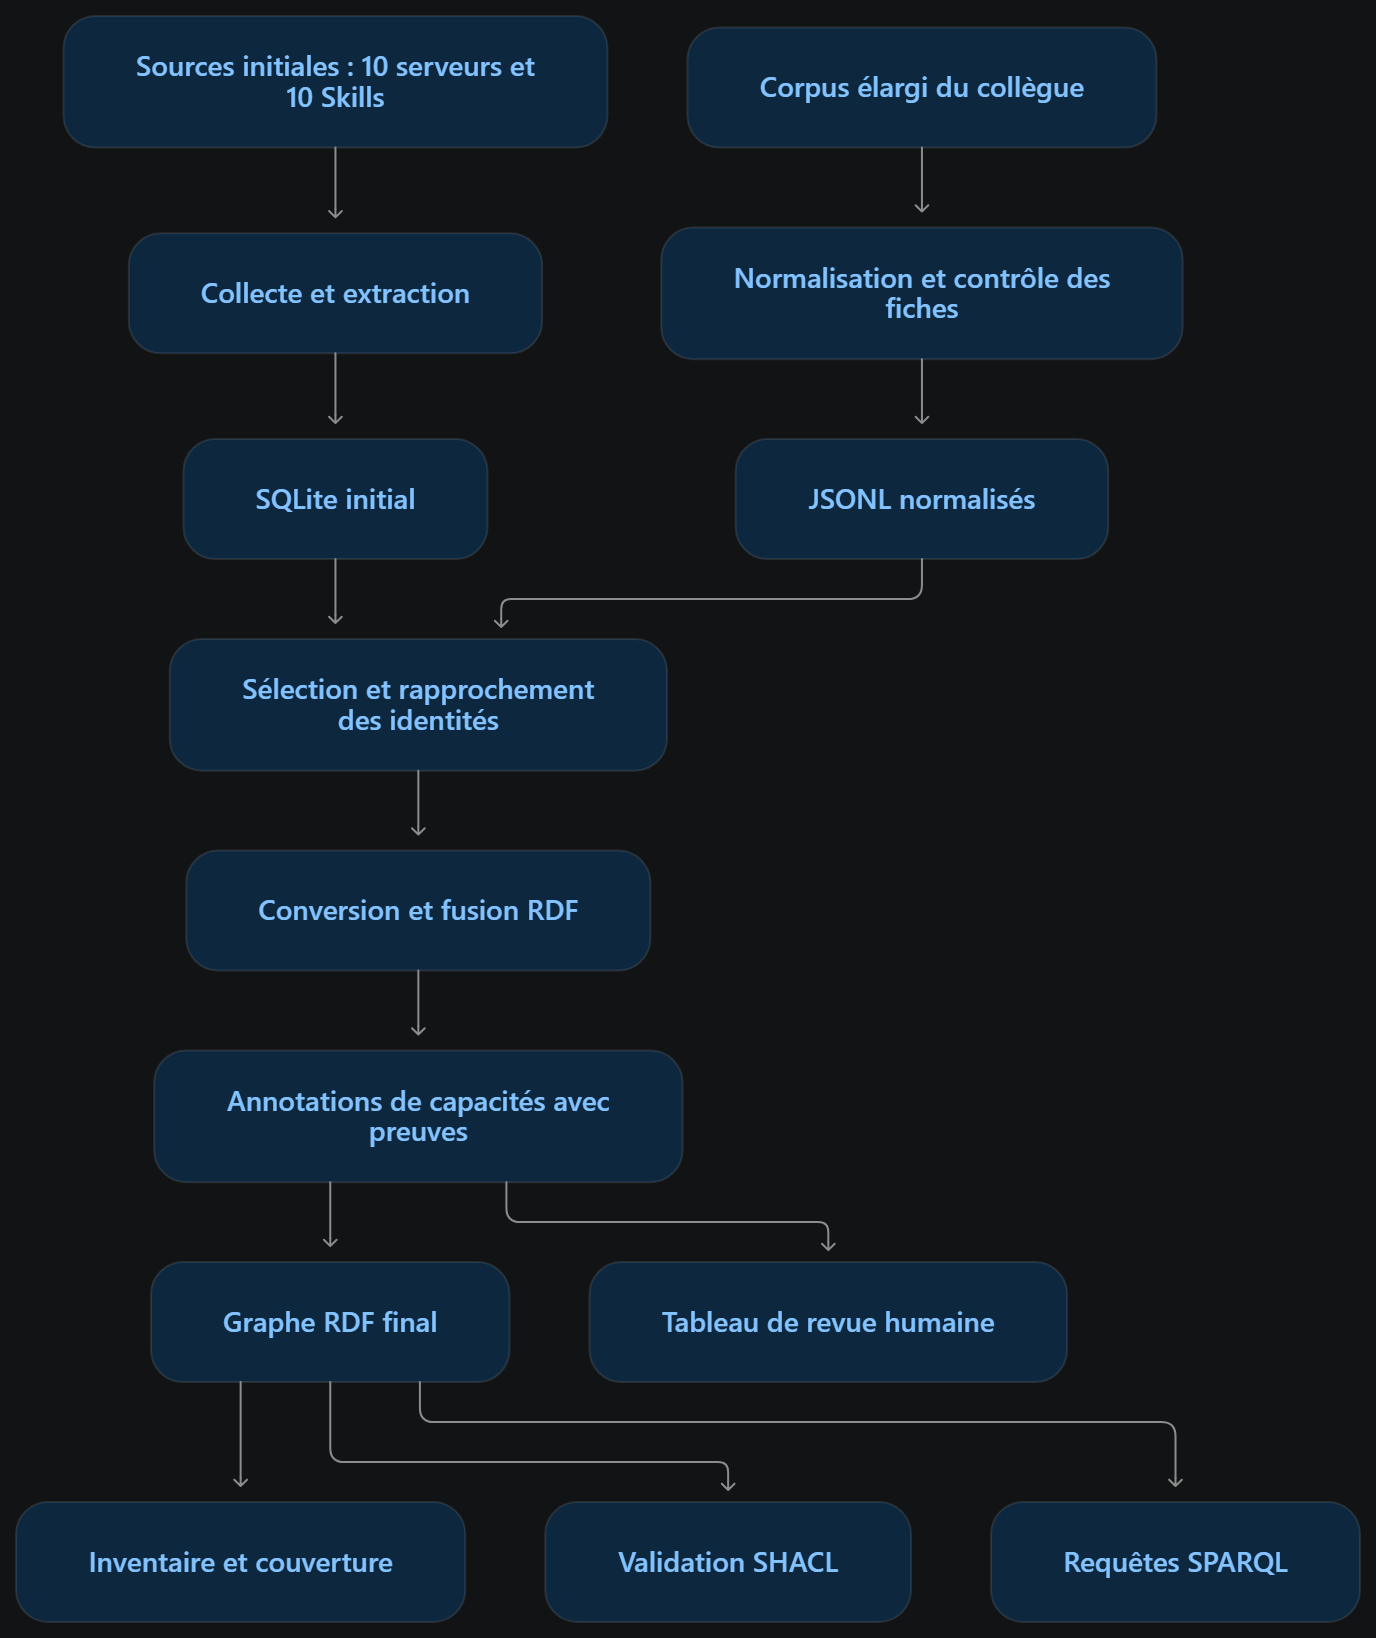
\includegraphics[width=\textwidth,height=0.65\textheight,keepaspectratio]{mermaid-diagram.png}
\caption{Workflow of the current pipeline, showing the selected sources, task annotations, discovery queries and validation reports.}
\label{fig:pipeline-workflow}
\end{figure}


\section{Remaining limitations and next steps}

The main result this week is a single reproducible graph connecting the selected sources, task annotations, discovery queries and validation reports. However, annotation coverage does not establish semantic accuracy, and the current metadata does not guarantee runtime availability or complete tool inventories.

My next step is to assess a manageable, varied sample of assertions, starting with the competency questions and less certain secondary-source records. I plan to record accept, correct, reject and investigate decisions persistently so that reconstruction preserves the review results. I will also refine overly broad task labels and investigate requirements that are absent from the available metadata. This will help evaluate the quality of the graph beyond its structural conformance.

\end{document}
